% !TeX document-id = {1d88a3b2-9b5b-461b-9b0a-590d1c20474b}
% !TeX TXS-program:compile = txs:///pdflatex/[--shell-escape]
\documentclass[border={0 0mm 0 -1mm}]{standalone}
\usepackage{amsmath,amsfonts,amssymb}
\usepackage{tikz,pgfplots}
\usetikzlibrary{arrows,arrows.meta,bending,calc,decorations,shadings,shadows,shapes,shapes.arrows,shapes.geometric}
\usetikzlibrary{calc,fadings,decorations.pathreplacing}
\usepgfplotslibrary{units,fillbetween,groupplots,colorbrewer}
\usetikzlibrary{pgfplots.colorbrewer,}
\usepackage{pgfplotstable}
\usetikzlibrary{3d,spy}
\usepgfmodule{plot}
\usepackage{scalerel}

\newcommand*{\xMin}{-2}%
\newcommand*{\xMax}{9}%
\newcommand*{\yMin}{-4}%
\newcommand*{\yMax}{6.5}%

\definecolor{As}{RGB}{255,255,0}
\definecolor{Al}{RGB}{173,216,230}
\definecolor{Ga}{RGB}{0,128,150}
\begin{document}
	
	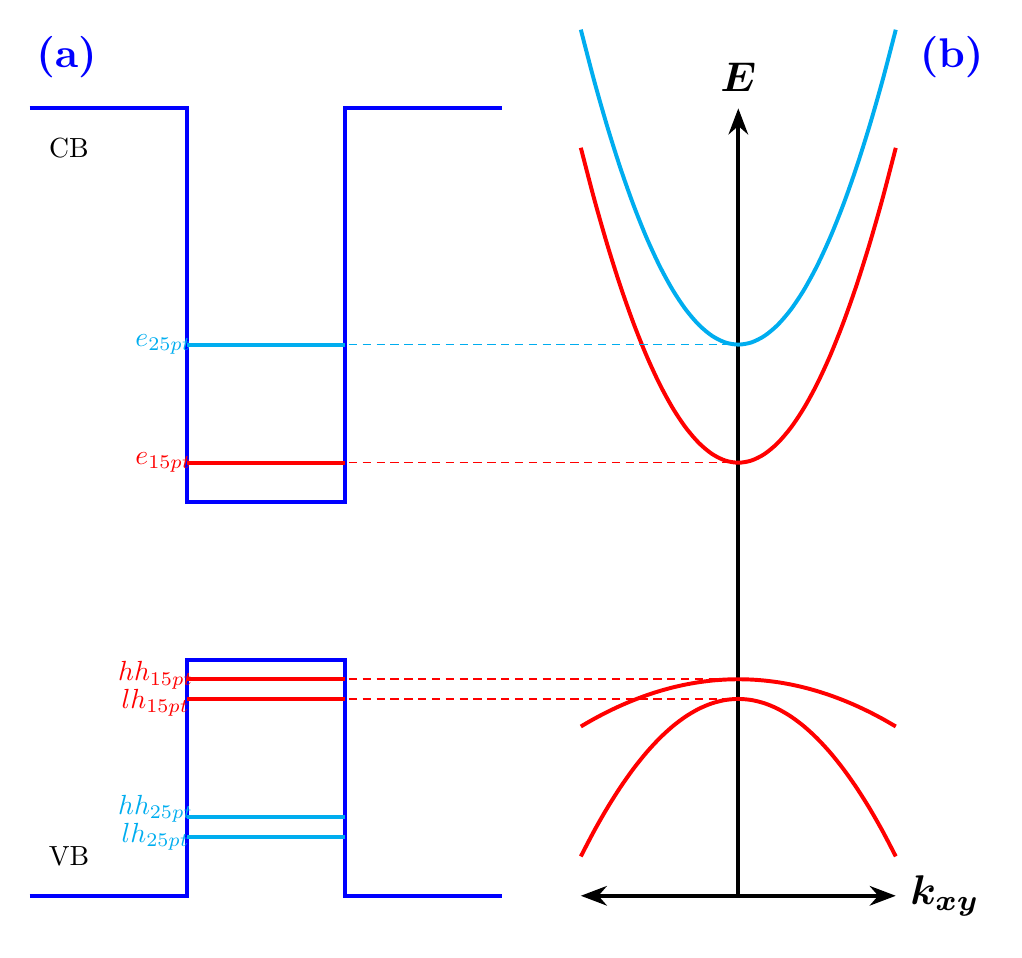
\begin{tikzpicture}
%	\draw[step=.5cm,gray,very thin,opacity=0.2] (0,0) grid (\xMax,\yMax);
%		\foreach \i in {\xMin,...,\xMax} {
%				\draw [very thin,gray,opacity=0.2] (\i,\yMin) -- (\i,\yMax)  node [below,opacity=1] at (\i,\yMin) {$\i$};
%													}
%			\foreach \i in {\yMin,...,\yMax} {
%					\draw [very thin,gray,opacity=0.2] (\xMin,\i) -- (\xMax,\i) node [left,opacity=1] at (\xMin,\i) {$\i$};
%						}
%				
		
		\begin{scope}[rotate=0,xshift=0cm,yshift=0cm]	
			%\draw[-{Triangle[width=3mm,length=7mm]}, line width=1mm,black](-2.3,-5) -- node[above,yshift=6cm,scale=2] {$E$} (-2.3, 7);
			%\draw[-{Triangle[width=3mm,length=7mm]}, line width=1mm,black](-2.35,-5) -- node[midway,xshift=4cm,scale=2] {$z$} (5, -5);
			\node[scale=1.5,font=\bf,anchor=north west,inner sep=0.5mm,text=blue] at (-2,7) {(a)};
			\node[scale=1.5,font=\bf,anchor=north east,inner sep=0.5mm,text=blue] at (10.2,7) {(b)};
			
			\node at (-1.5,5.5) {CB};
			\node at (-1.5,-3.5) {VB};

			\draw[line width=0.5mm,blue] (-2,6)--(0,6)--(0,1)--(2,1)--(2,6)--(4,6);
			\draw[line width=0.5mm,blue](-2,-4)--(0,-4)--(0,-1)--(2,-1)--(2,-4)--(4,-4);
			%\draw[fill=gray] (-2,2)--(0,2) parabola bend (1,3) (2,2)--(4,2);
			\draw[red,line width=0.5mm] (0,1.5)--(2,1.5);
			\draw[cyan,line width=0.5mm] (0,3)--(2,3);
			
			\draw[red,line width=0.5mm] (0,-1.25)--(2,-1.25);
			\draw[red,line width=0.5mm] (0,-1.5)--(2,-1.5);
			
			\draw[cyan,line width=0.5mm] (0,-3)--(2,-3);
			\draw[cyan,line width=0.5mm] (0,-3.25)--(2,-3.25);
			
		\draw[-{Stealth},line width=0.5mm] (7,-4)--node [above,yshift=5cm,scale=1.5] {$\boldsymbol{E}$}(7,6);
		\draw[{Stealth}-{Stealth},line width=0.5mm] (5,-4)--node[midway,scale=1.5,xshift=1.75cm] {$\boldsymbol{k_{xy}}$}(9,-4);
		\draw[ line width = 0.50mm,xshift=7cm,yshift=1.5cm,red]   plot[smooth,domain=-2:2] (\x, {\x*\x});
		\draw[cyan, line width = 0.50mm,xshift=7cm,yshift=3cm]   plot[smooth,domain=-2:2] (\x, {\x*\x});
		
		\draw[black, line width = 0.50mm,xshift=7cm,yshift=-1.25cm,red]   plot[smooth,domain=-2:2] (\x, {-0.15*\x*\x});
		\draw[black, line width = 0.50mm,xshift=7cm,yshift=-1.5cm,red]   plot[smooth,domain=-2:2] (\x, {-0.5*\x*\x});
		
		%Labels
		\draw[red, densely dashed,line width=0.2mm](1,1.5)--(7,1.5);
		\draw[cyan, densely dashed,line width=0.2mm](1,3)--(7,3);
		\draw[red, densely dashed,line width=0.2mm](1,-1.5)--(7,-1.5);
		\draw[red, densely dashed,line width=0.2mm](1,-1.25)--(7,-1.25);
		\node[red] at (-0.3,1.5) {$e_{\scaleto{1}{5pt}}$};	
	    \node[cyan] at (-0.3,3) {$e_{\scaleto{2}{5pt}}$};
	    \node[red] at (-0.4,-1.2) {$hh_{\scaleto{1}{5pt}}$};
	    \node[red] at (-0.4,-1.55) {$lh_{\scaleto{1}{5pt}}$}; 
	    \node[cyan] at (-0.4,-2.9) {$hh_{\scaleto{2}{5pt}}$};
	    \node[cyan] at (-0.4,-3.25) {$lh_{\scaleto{2}{5pt}}$};

	    
		

	\end{scope}
		
		
	
	\end{tikzpicture}
	
	
\end{document}